\documentclass{article}\usepackage{graphicx, color}
%% maxwidth is the original width if it is less than linewidth
%% otherwise use linewidth (to make sure the graphics do not exceed the margin)
\makeatletter
\def\maxwidth{ %
  \ifdim\Gin@nat@width>\linewidth
    \linewidth
  \else
    \Gin@nat@width
  \fi
}
\makeatother

\definecolor{fgcolor}{rgb}{0.2, 0.2, 0.2}
\newcommand{\hlnumber}[1]{\textcolor[rgb]{0,0,0}{#1}}%
\newcommand{\hlfunctioncall}[1]{\textcolor[rgb]{0.501960784313725,0,0.329411764705882}{\textbf{#1}}}%
\newcommand{\hlstring}[1]{\textcolor[rgb]{0.6,0.6,1}{#1}}%
\newcommand{\hlkeyword}[1]{\textcolor[rgb]{0,0,0}{\textbf{#1}}}%
\newcommand{\hlargument}[1]{\textcolor[rgb]{0.690196078431373,0.250980392156863,0.0196078431372549}{#1}}%
\newcommand{\hlcomment}[1]{\textcolor[rgb]{0.180392156862745,0.6,0.341176470588235}{#1}}%
\newcommand{\hlroxygencomment}[1]{\textcolor[rgb]{0.43921568627451,0.47843137254902,0.701960784313725}{#1}}%
\newcommand{\hlformalargs}[1]{\textcolor[rgb]{0.690196078431373,0.250980392156863,0.0196078431372549}{#1}}%
\newcommand{\hleqformalargs}[1]{\textcolor[rgb]{0.690196078431373,0.250980392156863,0.0196078431372549}{#1}}%
\newcommand{\hlassignement}[1]{\textcolor[rgb]{0,0,0}{\textbf{#1}}}%
\newcommand{\hlpackage}[1]{\textcolor[rgb]{0.588235294117647,0.709803921568627,0.145098039215686}{#1}}%
\newcommand{\hlslot}[1]{\textit{#1}}%
\newcommand{\hlsymbol}[1]{\textcolor[rgb]{0,0,0}{#1}}%
\newcommand{\hlprompt}[1]{\textcolor[rgb]{0.2,0.2,0.2}{#1}}%

\usepackage{framed}
\makeatletter
\newenvironment{kframe}{%
 \def\at@end@of@kframe{}%
 \ifinner\ifhmode%
  \def\at@end@of@kframe{\end{minipage}}%
  \begin{minipage}{\columnwidth}%
 \fi\fi%
 \def\FrameCommand##1{\hskip\@totalleftmargin \hskip-\fboxsep
 \colorbox{shadecolor}{##1}\hskip-\fboxsep
     % There is no \\@totalrightmargin, so:
     \hskip-\linewidth \hskip-\@totalleftmargin \hskip\columnwidth}%
 \MakeFramed {\advance\hsize-\width
   \@totalleftmargin\z@ \linewidth\hsize
   \@setminipage}}%
 {\par\unskip\endMakeFramed%
 \at@end@of@kframe}
\makeatother

\definecolor{shadecolor}{rgb}{.97, .97, .97}
\definecolor{messagecolor}{rgb}{0, 0, 0}
\definecolor{warningcolor}{rgb}{1, 0, 1}
\definecolor{errorcolor}{rgb}{1, 0, 0}
\newenvironment{knitrout}{}{} % an empty environment to be redefined in TeX

\usepackage{alltt}
\usepackage{amsmath,amsfonts,bm,fullpage,multirow}
\usepackage{natbib}
\bibliographystyle{abbrvnat}
\newcommand{\ProjMean}{{\widehat{\bm S}_{2}}}
\newcommand{\ProjMedian}{{\widehat{\bm S}_{1}}}
\newcommand{\HuberMean}{{\widehat{\bm S}_H}}
\newcommand{\R}{{\mathbb{R}}}
\IfFileExists{upquote.sty}{\usepackage{upquote}}{}
\begin{document}

\begin{center}
\Large{\bf Robustifying the Projected Mean}
\end{center}
\normalsize
This is the literature I have found methods to robustify the $L_2$ estimator for various data types.  Specifically I focus on the trimmed and winsorized means.



 
\section{Trimmed Means}

Assume the sample of size $n$, $x_1,\dots,x_n$, has empirical distribution function $F_n$.  The sample $\alpha$-trimmed mean, according to \cite{huber2009} page 10, is
\[
\bar{X}_\alpha=\frac{1}{1-2\alpha}\int_{\alpha}^{1-\alpha}F_n^{-1}(t)dt.
\]

The following is taken from Section 4 of \cite{laha2011}. In the circular context, suppose $\theta$ is a circular random variable with p.d.f.~$f(\theta)$ and $0<\gamma\leq 0.5$ is fixed.  Let $\alpha,\beta$ be two points on the unit circle satisfying
\[
\int_{\beta}^\alpha f(\theta)d\theta=1-2\gamma.
\] 
The circular $\gamma$-trimmed mean is
\[
\mu_\gamma=\text{arg}\left[\frac{1}{1-2\gamma}\int^{\alpha}_\beta\exp(\imath\theta)f(\theta)d\theta\right].
\]
In their Theorem 4.1 they show it is SB-robust for the circular von Mises distribution.  In \cite{laha2013} they show it is SB-robust for the wrapped normal distribution too.  Remember SB-robustness is always with respect to some dispersion measure.




\section{Weighted Means}

According to \cite{huber2009} Section 11.2.2 the current best possible break down for a $d$-dimensional affine equivalent estimator is
\[
\epsilon^*=\frac{n-2d+1}{2n-2d+1}.
\]
So for us, this would be $(n-5)/(2n-5)$.  This break-down is achieved by the weighted average of the points $\bm x_i$ from $\bm X$ with weights $w_i=w(r_i)$ where
\[
r_i=\sup_{\bm u}\frac{\bm u^\top\bm x_i-\text{MED}(\bm u^\top\bm X)}{\text{MAD}(\bm u^\top\bm X)}
\]
and $w(r)$ is a strictly positive, decreasing function of $r\geq 0$, with $w(r)r$ bounded.  I think $r_i$ can be replaced with any one-dimensional projection of the outlyingness of the $\bm x_i$.  For example, $H_n$ or the distance the mean moves when $\bm R_i$ is removed.







\section{Huber Estimator}

The multidimensional Huber estimator \citep{hampel2011} places a upper-bound on the influence function.  For observations beyond that bound, that point is projected into that bound. In the strict definition (4.3.2 on page 239) they bound the influence function.  Since the influence function of $\ProjMean$ is
\[
\text{IF}_2(\bm R_i,F)=\frac{3}{1+2E[\cos(r)]}\sin(r)\bm u
\]
then all that is being bounded is $\sin(r)$.  

Unfortunately, this is not a very good estimator for us because it puts the most restrictions on the range near $\pi/2$ instead or $\pi$.  Therefore the modified Huber estimator on $SO(3)$ puts a bound on $r_i=d_r(\bm R_i,\ProjMean)$ and is denoted $\HuberMean$.

The algorithm I use to compute $\HuberMean$ based on the sample $\bm R_1,\dots,\bm R_n$ and the constant $c<\pi$ is as follows
\begin{enumerate} 
\item Compute $\ProjMean^{(j)}$
\item For each $i$ compute $r_i^{(j)}=d_r(\bm R_i,\ProjMean^{(j)})$
\item For each $i$ such that $r_i>c$:
\begin{enumerate}
\item Find $\bm u_i\in\mathcal{S}^3$ satisfying $\exp[\bm{\Phi}(r_i\bm u_i)]=\ProjMean^{(j)\top}\bm R_i$
\item Redefine $\bm R_i=\ProjMean^{(j)\top}\exp[\bm{\Phi}(c\bm u_i)]$
\end{enumerate}
\item Repeat steps 1 - 3 for $j+1$ until $\ProjMean^{(j)\top}\ProjMean^{(j+1)}\approx \bm{I}_{3\times 3}$
\item Define $\HuberMean=\ProjMean^{(j+1)}$
\end{enumerate}

The winsorized mean is similar, but instead of specifying a certain distance after which the observation is projected closer, one specifies a certain percentage of the points that will be projected closer.  To order the data the square root of the $H_n$ statistic discussed above is used, that is for each $i$ $H_n$ is computed and the square root is taken.  The upper $1-\alpha$\% percentage is projected the the inner circle maintaining their original axis of rotation, but the angle of rotation is changed to the appropriate percentile.

% 
% Thus the gross error sensitivity is
% \[
% \|\text{IF}_2(\bm R_i,F)\|=\|\frac{3}{1+2E[\cos(r)]}\sin(r)\bm u\|=\left|\frac{3\sin(r)}{1+2E[\cos(r)]}\right|=\frac{3\sin(|r|)}{1+2E[\cos(r)]}
% \]








\section{(Very) Limited Simulation Study}

I ran a very small simulation study with the new robustified $\ProjMean$ estimators (trimmed, winsorized, weighted, Huber) along with the tradition $\ProjMean$ and $\ProjMedian$.  I generated 100 samples per combination of distribution (Cayley or von Mises Fisher), sample size ($n=10,50$), concentration ($\kappa=0.5,1,10$) all with $10\%$ contamination.  Meaning 90\% of each sample was from the $F(\bm I_{3\times 3},\kappa)$ distribution and 10\% of the sample came from a $F(\bm S_c[\pi/2,\bm u],\kappa)$, i.e.~the slippage situation where the second principal direction was rotation though $\pi/2$ radians about some (uniformly distributed) axis.

In Table \ref{tab:SimRes} is the average bias based on the Euclidean distance in each estimator for each simulated scenario.  That is bias$=\|\bm I_{3\times 3}-\widehat{\bm S}\|_F$ for each estimator.  The trimmed and winsorized mean use $\alpha=0.1$ and the Huber estimator sets $c=0.75$.





\begin{table}[ht]
\centering
\begin{tabular}{lrrrrrrrr}
  \hline
  Dist& n & $\kappa$  & Mean & Median & Trim & Winz & Weight &Huber\\ 
  \hline
  & &0.50  & 1.46 & 1.64 & 1.52 & 1.45 & 1.51 & 1.45 \\
  & 10&1.00  & 1.06 & 1.30 & 1.11 & 1.04 & 1.15 & 1.05 \\ 
 \multirow{2}{*}{Cayley} & &10.00  & 0.35 & 0.38 & 0.35 & 0.36 & 0.35 & 0.35 \\ \cline{2-9}
  & &0.50 & 0.81 & 0.97 & 0.85 & 0.77 & 0.87 & 0.78 \\ 
  & 50&1.00  & 0.51 & 0.64 & 0.53 & 0.47 & 0.56 & 0.49 \\
  & &10.00 & 0.21 & 0.18 & 0.16 & 0.20 & 0.19 & 0.19 \\ \hline
  
  & &0.50 & 0.70 & 0.48 & 0.72 & 0.71 & 0.58 & 0.69 \\ 
  & 10&1.00  & 0.49 & 0.32 & 0.52 & 0.51 & 0.38 & 0.46 \\
 \multirow{2}{*}{von Mises} & &10.00& 0.20 & 0.09 & 0.14 & 0.18 & 0.12 & 0.17 \\ \cline{2-9}
  & &0.50   & 0.30 & 0.14 & 0.31 & 0.31 & 0.20 & 0.29 \\ 
  & 50&1.00 & 0.27 & 0.11 & 0.28 & 0.27 & 0.17 & 0.25 \\ 
  & &10.00 & 0.17 & 0.03 & 0.06 & 0.12 & 0.07 & 0.12 \\
   \hline
\end{tabular}
\caption{Mean estimator bias based on 100 samples from each combination of distribution, sample size and concentration.}
\label{tab:SimRes}
\end{table}

\begin{figure}
\centering
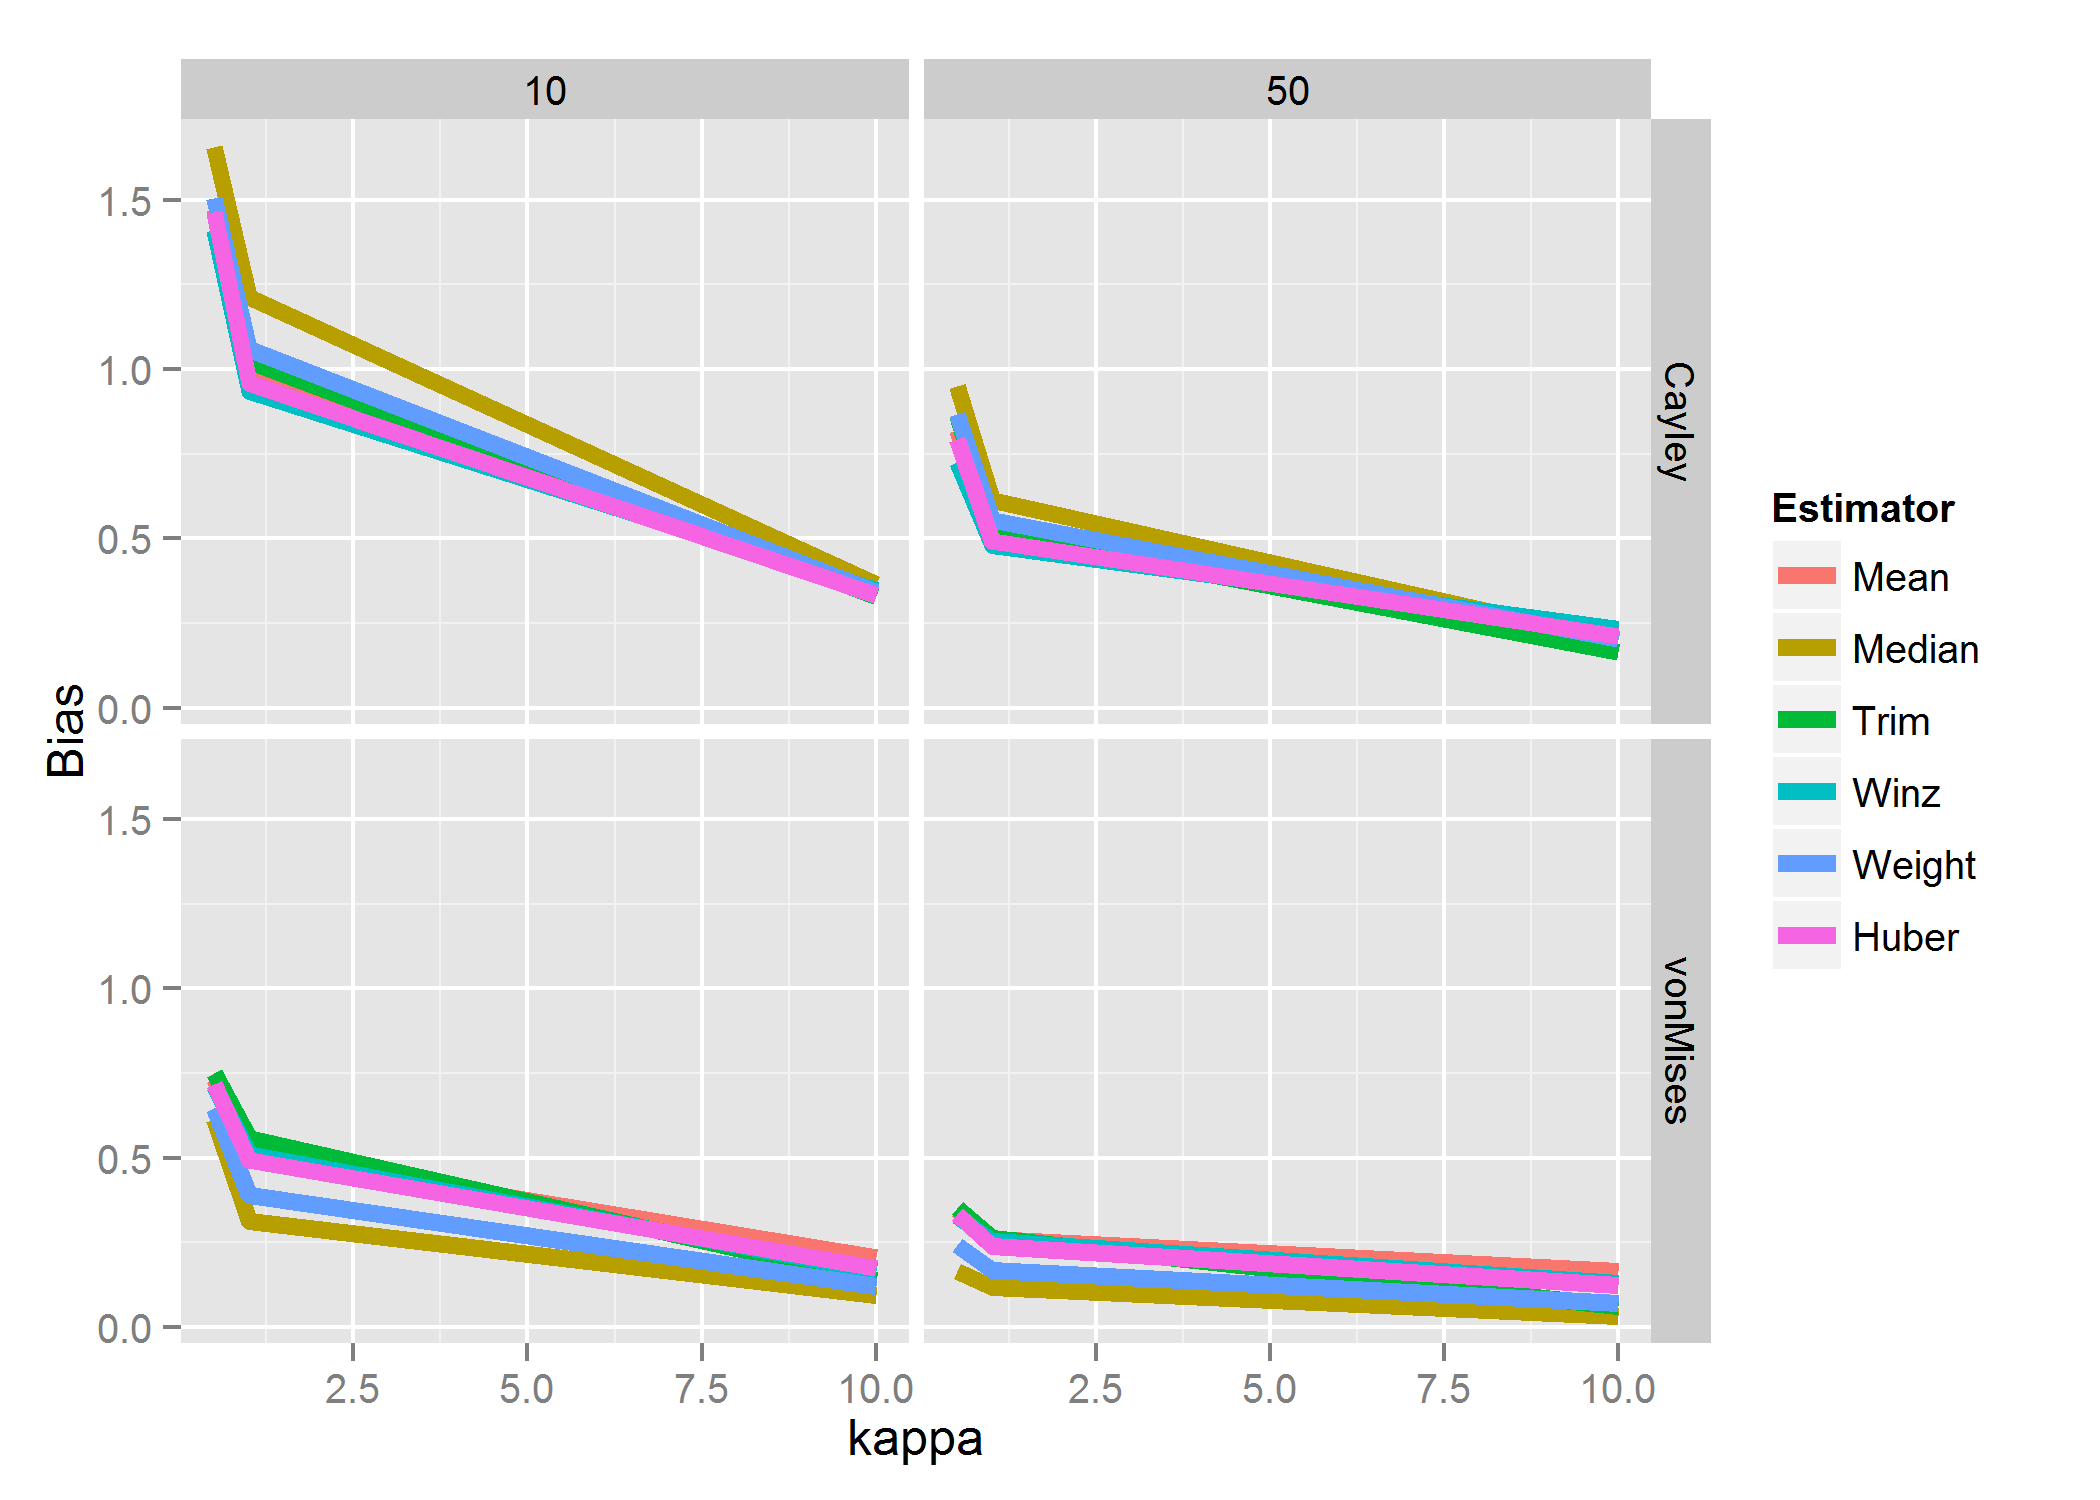
\includegraphics[width=.7\textwidth]{Estimator.png}
\caption{Graphical representation of Table \ref{tab:SimRes} faceted by distribution and sample size.}
\end{figure}

It looks like the median is unbeatable for the von Mises Distribution.
\clearpage
%\bibliographystyle{plain}
\bibliography{../OutlierDetection/RobustRefs}
\end{document}
